 \documentclass[sigconf]{acmart}
\usepackage{booktabs} % For formal tables
\usepackage{amsmath,amssymb,amsfonts}
\usepackage{algorithmic}
\usepackage{algorithm}
\usepackage{graphicx}
\usepackage{textcomp}
\usepackage{xcolor}
\usepackage{epstopdf}
\usepackage{secdot}
\sectiondot{section}
\usepackage{caption}
\usepackage{booktabs}
\captionsetup{skip=2pt}
\usepackage{subcaption}
\usepackage{framed}
%\usepackage[font=small,skip=0pt]{caption}
\usepackage[referable]{threeparttablex}
\usepackage{multirow,array}
\usepackage{color}

\newcommand{\tabincell}[2]{\begin{tabular}{@{}#1@{}}#2\end{tabular}}

\def\UrlBreaks{\do\/\do-}
\renewcommand{\UrlBreaks}{\do\/\do-\do:\do_\do\a\do\b\do\c\do\d\do\e\do\f\do\g\do\h\do\i\do\j\do\k\do\l\do\m\do\n\do\o\do\p\do\q\do\r\do\s\do\t\do\u\do\v\do\w\do\x\do\y\do\z\do\A\do\B\do\C\do\D\do\E\do\F\do\G\do\H\do\I\do\J\do\K\do\L\do\M\do\N\do\O\do\P\do\Q\do\R\do\S\do\T\do\U\do\V\do\W\do\X\do\Y\do\Z}

% Disable / remove copyright boxes
\setcopyright{none}
\settopmatter{printacmref=false}
\renewcommand\footnotetextcopyrightpermission[1]{}

% Increase margin between text and footer
\setlength{\footskip}{20pt}

% Add CCR footer
\usepackage{fancyhdr}
\fancypagestyle{plain}{%
   \fancyhf{} %
   \fancyfoot[L]{ACM SIGCOMM Computer Communication Review}%
   \fancyfoot[R]{Volume 49 Issue 3, July 2019}%
}
\pagestyle{plain}
% Add CCR footer on first page
\fancypagestyle{firstpagestyle}{%
   \fancyhf{} %
   \fancyfoot[L]{ACM SIGCOMM Computer Communication Review}%
   \fancyfoot[R]{Volume 49 Issue 3, July 2019}%
}
\usepackage{balance}

\begin{document}
\title{Towards Passive Analysis of Anycast in Global Routing: Unintended Impact of Remote Peering}

\author{Rui Bian}
\affiliation{
	\institution{University of Delaware}
}\email{bianrui@udel.edu}

\author{Shuai Hao}
\affiliation{
	\institution{CAIDA / UC San Diego}
}\email{haos@caida.org}

\author{Haining Wang}
\affiliation{
	\institution{University of Delaware}
}\email{hnw@udel.edu}

\author{Amogh Dhamdere}
\affiliation{
	\institution{CAIDA / UC San Diego}
}\email{amogh@caida.org}

\author{Alberto Dainotti}
\affiliation{
	\institution{CAIDA / UC San Diego}
}\email{alberto@caida.org}

\author{Chase Cotton}
\affiliation{
	\institution{University of Delaware}
}\email{ccotton@udel.edu}

%!TEX root = main_acm.tex

\begin{abstract}
Anycast has been widely adopted by today's Internet services, including DNS, CDN, and DDoS protection, in which the same IP address is announced from distributed locations and clients are directed to the topologically-nearest service replica. Prior research has focused on various aspects of anycast, either its usage in particular services such as DNS or characterizing its adoption by Internet-wide active probing methods. In this paper, we first explore an alternative approach to characterize anycast based on previously collected global BGP routing information. 
Leveraging state-of-the-art active measurement results as near-ground-truth, our passive method without requiring any Internet-wide probes can achieve 90\% accuracy in detecting anycast prefixes. More importantly, our approach uncovers anycast prefixes that have been missed by prior datasets based on active measurements.
While investigating the root causes of inaccuracy, we reveal that anycast routing has been entangled with the increased adoption of remote peering, a type of layer-2 interconnection where an IP network may peer at an IXP remotely without being physically present at the IXP. The invisibility of remote peering from layer-3 breaks the assumption of the shortest AS paths on BGP and causes an unintended impact on anycast performance. We identify such cases from BGP routing information and observe that at least 19.2\% of anycast prefixes have been potentially impacted by remote peering.
\end{abstract}


\begin{CCSXML}
<ccs2012>
<concept>
<concept_id>10003033.10003039.10003045.10003046</concept_id>
<concept_desc>Networks~Routing protocols</concept_desc>
<concept_significance>500</concept_significance>
</concept>
<concept>
<concept_id>10003033.10003099.10003104</concept_id>
<concept_desc>Networks~Network management</concept_desc>
<concept_significance>300</concept_significance>
</concept>
<concept>
<concept_id>10003033.10003106.10010924</concept_id>
<concept_desc>Networks~Public Internet</concept_desc>
<concept_significance>300</concept_significance>
</concept>
</ccs2012>
\end{CCSXML}

\ccsdesc[500]{Networks~Routing protocols}
\ccsdesc[300]{Networks~Network management}
\ccsdesc[300]{Networks~Public Internet}

\keywords{Internet Routing, Anycast, Peering, Remote Peering}

\maketitle

%!TEX root = main_acm.tex

\section{Introduction}\label{sec:intro}

IP anycast is widely used in modern Content Delivery Networks (CDNs)~\cite{Calder:2015}, Domain Name
System (DNS)~\cite{fan2013,moura2016anycast},
and Distributed Denial of Service (DDoS) protections~\cite{moura2016anycast}. 
With anycast, the same IP address(es) is announced from multiple locations, and the Border Gateway Protocol (BGP) is responsible for directing clients to the site that is the ``closest'' to them on the basis of ``best routing'' (i.e., AS path), providing reduced latency and improved availability to end-users.

In recent years, researchers have conducted studies to understand and
characterize anycast from various angles, such as its adoption~\cite{cicalese2015characterizing} or the efficiency in particular services like DNS~\cite{li2018internet}.
Due to the insufficient distinctions between unicast and anycast from the perspective of a routing table, the common method to identify anycast addresses is through {\it active} Internet-wide measurements.
Cicalese \emph{et al.}~\cite{cicalese2015characterizing, cicalese2015fistful} studied the enumeration and city-level geolocation of anycast prefixes by using latency measurements based on the detection of speed-of-light violations. 
However, the latency of ping may not always reliably reflect the geographic
distance of two IP addresses~\cite{pam02, Zhang:2005}. Also, active probing requires the use of many vantage points to achieve the necessary coverage.

To overcome these limitations, in this work, we explore a passive approach to
identify and characterize IP anycast by leveraging BGP routing information.
Specifically, we propose and analyze a set of BGP-related features to classify
anycast and unicast prefixes, and utilize simple classifiers to train and
predict anycast prefixes on the Internet. The results demonstrate that our
passive approach, without requiring probing, can achieve 90\% accuracy.
Furthermore, we delve into the instances misclassified by our approach to find the
root causes of inaccuracy.

The two major assumptions of our approach are that (1) anycast prefixes may have more upstream autonomous systems (ASes) than unicast prefixes, as anycast is announced from multiple physical locations and peering with transit providers at different places, and (2) the distance between such upstream ASes will be topologically larger than that in the scenarios of unicast prefixes (i.e., more hops in AS paths), as some of them are geographically distant from others. However, in our false positives, we also find some unicast prefixes falling into such a category. Through a deeper analysis, we identify that many of these cases involve {\it remote peering}~\cite{castro2014remote, Nomikos18}. 
 
Remote peering allows a network to peer at an Internet exchange point (IXP) without a physical presence within the IXP's infrastructure, either over a long cable or over IXP's reseller partners that provide IXP layer-2 access. Remote peering enables the fast deployment of connectivity to an IXP and reduces cost. However, it also brings unintended impact on global routing due to its invisibility at layer-3, breaking the assumption that the peered autonomous systems are physically close and provide a short path for transporting traffic. As such, we investigate the impact of remote peering on anycast routing by using passive methods and validate our analysis through traceroute results. 


The remainder of this paper is organized as follows. We introduce the background of anycast and remote peering \S \ref{sec:back}. We present our methodology to identify anycast prefixes in \S\ref{sec:meth}. We investigate inaccuracies in our method in \S\ref{sec:inaccu} and the impact of remote peering on anycast routing in \S\ref{sec:rp}. We survey related work in \S\ref{sec:rel} and conclude the paper in \S\ref{sec:con}.



%!TEX root = main_acm.tex

\section{Background}
\label{sec:back}

\subsection{BGP and Anycast}

Border Gateway Protocol (BGP) \cite{rekhter2005border} is the de facto
inter-domain routing protocol, designed to exchange reachability information
among autonomous systems on the Internet. BGP selects a best AS path based on various attributes (e.g., the shortest path) to reach the specific destination.

Anycast \cite{abley2006operation} is a network addressing and routing methodology by which a collection of servers announce the same IP address from multiple geographically distributed sites. 
As routers usually choose the shortest AS path, the user requests sent to an anycast address are routed to the topologically nearest endpoint. 
As a result, anycast has many advantages over unicast such as reduced latency, load balancing, DDoS mitigation, and improved robustness.

\subsection{Remote Peering}  
Peering is a relationship where two networks exchange traffic directly rather than through a transit provider.
Remote peering~\cite{castro2014remote, Nomikos18} is a new peering type where a
network peers at an IXP through layer-2 remote peering providers such as resellers without a physical presence in the IXP's infrastructure. Fig. \ref{RP} shows an example of remote peering. 
Remote peering can be implemented with standard methods like MPLS
(Multi-Protocol Label Switching) and VPNs (Virtual Private Networks) in layer-2,
and provide benefits such as low cost, increased connectivity, and easy
management. Nevertheless, it also has some drawbacks such as degradation of
performance, loss of resilience, and difficulty for layer-3 management~\cite{Nomikos18}.
Furthermore, due to the invisibility at layer-3, BGP routers are not aware of
remote peering and may select as the shortest path a route where the actual endpoints are far from one another.

\begin{figure}[thbp]
\centerline{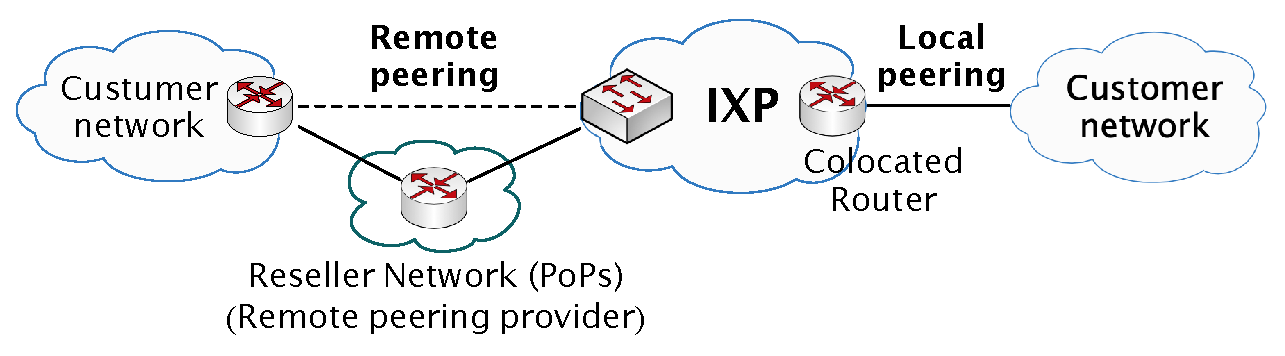
\includegraphics[scale=0.39]{fig/remote_peering.eps}}
\vspace{6pt}
\caption{Local and Remote Peering Models}
\label{RP}
\end{figure}
\vspace{-3pt}

%!TEX root = main_acm.tex

\section{Methodology}
\label{sec:meth}
In this section, we describe the datasets and the features we propose to extract from passively-collected BGP data for the purpose of identifying anycast routing. Using a reference dataset as {\it near}-ground-truth, we characterize the behavior of such BGP-related features in the wild. We then employ standard classification methods, decision tree and random forest, to train and evaluate the effectiveness of our approach for anycast detection using our proposed classification features. The repository including scripts and data used in our study is available at \cite{ccr_anycast}.

\subsection{Datasets}
\label{sec:data}
\subsubsection*{BGP Routing Information.} The datasets we used to detect and
characterize anycast prefixes are from the RouteViews project~\cite{Routeviews}
and RIPE's Routing Information Service (RIS)~\cite{RIPE_RIS}. 
In RouteViews and RIPE RIS, servers receive BGP information by peering with other BGP routers, often at large IXPs. We use CAIDA's BGPStream \cite{orsini2016bgpstream} to collect and process the data from RouteViews and RIPE RIS.

\subsubsection*{Anycast Dataset.} 
\label{sec:anycast_ground}
We use the anycast prefix list obtained through active measurements by Cicalese et al.~\cite{cicalese2015characterizing} as {\it near}-ground-truth, which provides a {\it conservative} estimation of Internet anycast usage.
The detection method in \cite{cicalese2015characterizing} is based on speed-of-light violations: if the latency measurements from multiple vantage points towards the same target exhibit geo-inconsistency, the target is  classified as anycast. They validated their method and scrutinized the dataset they make publicly available~\cite{DarioAnycastData} using ground-truth collected through protocol-specific techniques (e.g., DNS CHAOS requests or DPI over HTTP). 

However, we also notice that some prefixes strongly suggested as anycast by our method are not included in their dataset. We manually check and, through traceroute measurements, verify that most of them are indeed anycast prefixes. 
%Anycast prefixes missed by our method mostly belong to Microsoft, Google, CDNs and anycast-based DNS providers. The details are shown in \S\ref{sec:inaccu}. 

\begin{figure*}[th]
	\centerline{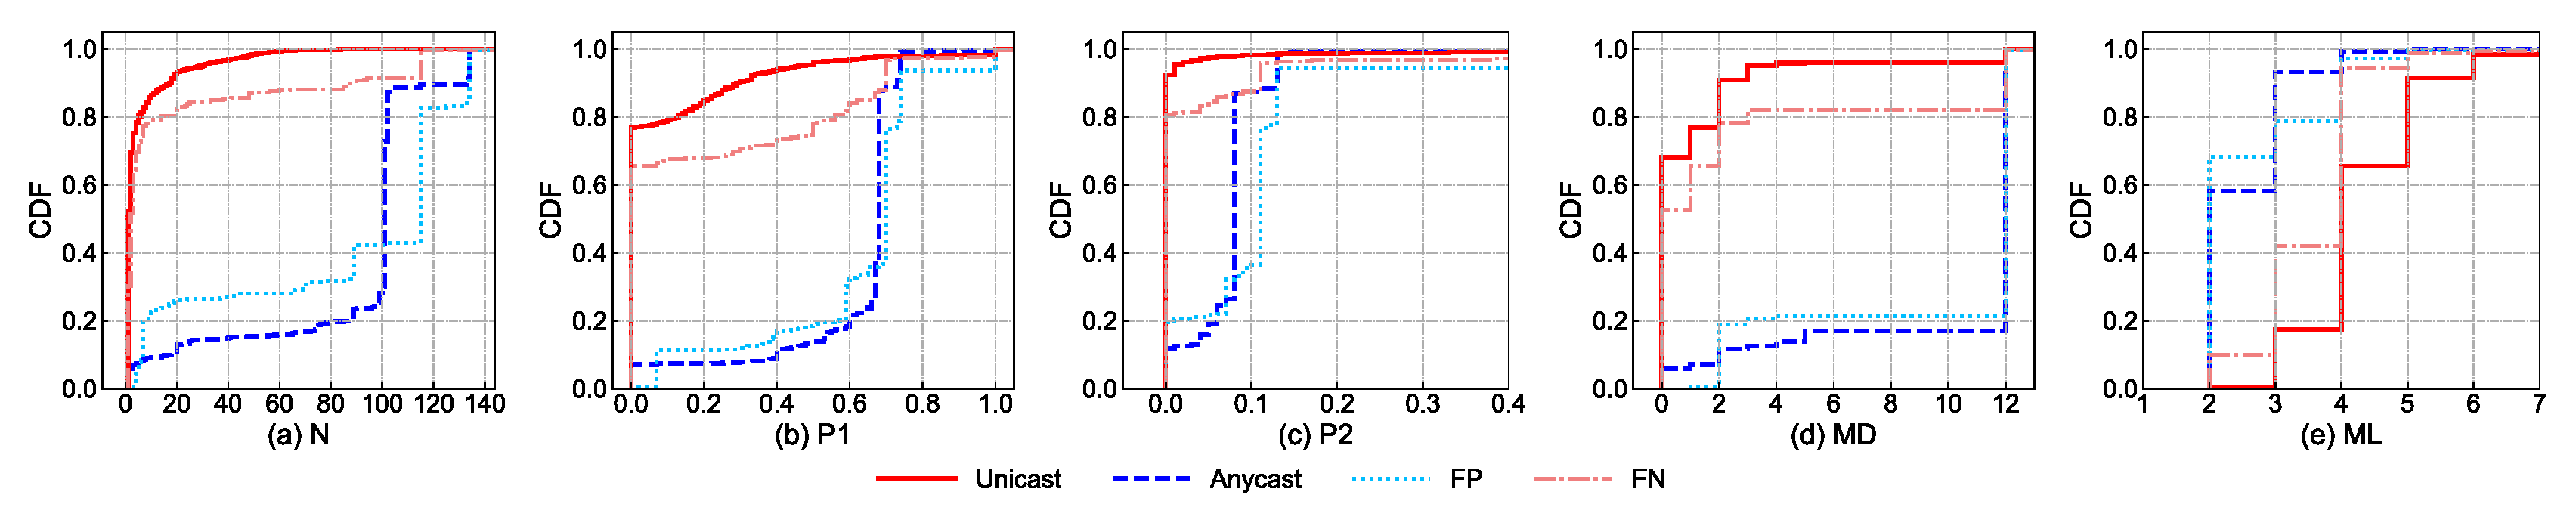
\includegraphics[scale=0.312]{fig/features.eps}}
	\vspace{3pt}
	\caption{ Distributions of the 5 classification features we propose for (1) anycast/unicast from the near-ground-truth dataset (\S\ref{feature}) and (2) False Positives/False Negatives from our passive classification (\S\ref{sec:inaccu})}
	\label{fig_FP_FN}
\end{figure*}

\subsection{BGP-related Features}

Due to the different deployment patterns between anycast and unicast, we leverage BGP routing information to characterize anycast prefixes. We propose and explore the following BGP-related features that could be used to identify anycast prefixes: as an anycast prefix is announced from multiple locations, some of its peer ASes should not be close to one another, both geographically and topologically.

\vspace{2pt}
\textbf{\texttt{N} - Number of upstream ASes:} We count the number of unique
\textit{upstream} ASes of each prefix. Given a prefix announced by $AS_{n}$, we
define \textit{upstream} ASes as the set of $AS_{n}$'s neighbor ASes that are
connected to $AS_{n}$ with either a customer-to-provider relationship (i.e.,
$AS_{n}$'s transit providers) or a peer-to-peer relationship, according to CAIDA's AS Relationships Dataset~\cite{as-rel}.

\textbf{\texttt{P1} - Percentage of upstream AS pairs whose distance is more than 1:}  We define the \textit{distance between two ASes} as the least number of AS hops between them in the observed paths.
For each prefix, we construct all the AS pairs between its upstream AS neighbors and label the number of AS pairs as $P$. We then identify the fraction of those AS pairs whose distance   is more than one, i.e., $P1=\ P_{dist>1}/ \ P$. 

\textbf{\texttt{P2} - Percentage of upstream-AS pairs whose distance is more than 2:} Similarly, P2 is defined as the fraction of those AS pairs with distance more than two, i.e., $P2=\ P_{dist>2}/ \ P$. Note that we propose P1 and P2 based on the assumption that the upstream ASes of an anycast prefix are more likely to be remote, both geographically and topologically.

\textbf{\texttt{MD} - Maximum distance between upstream ASes:} MD is the largest distance of two upstream ASes of a prefix. This variable tries to capture that upstream ASes for anycast prefixes are more spread out compared to unicast.

\textbf{\texttt{ML} - Maximum length of AS paths:} ML represents the length of
the longest AS path observed for a prefix. AS paths towards anycast prefixes
tend to be shorter, since they are announced from multiple locations. 

\subsection{Feature Validation}
\label{feature}

Given the features we proposed in \S3.2, we explore their potential for identifying anycast prefixes by analyzing their behavior with respect to prefixes labeled in the {\it near}-ground-truth dataset.  

\vspace{2pt}
\textbf{\texttt{N} }: Figure~\ref{fig_FP_FN}(a) shows the distributions of the number of upstream ASes, where we can see that the two classes of prefixes are clearly distinguishable from each other. Most anycast prefixes (90.2\%) have more than 17 upstream ASes, while 69.5\% of unicast prefixes only have one or two upstream ASes. This is consistent with the intuition that the routes towards an anycast prefix would be highly varied due to the geographically distributed deployment. 

\vspace{2pt}
\textbf{\texttt{P1}}: 
Figure~\ref{fig_FP_FN}(b) shows the distributions of P1. Obviously, P1 of
anycast prefixes is much larger than P1 of unicast prefixes. Specifically, P1 is
greater than 0.33 for 91.9\% of anycast prefixes,  and smaller than 0.07 for 78.1\% of unicast prefixes. A larger P1 for anycast prefixes implies that the upstream ASes are relatively far from one another because the upstream ASes of an anycast prefix are more geographically and topologically distributed. %\vspace{2pt}

\vspace{2pt}
\textbf{\texttt{P2}}: 
Similar to P1, from Figure~\ref{fig_FP_FN}(c), P2 is smaller than 1\% for 95.4\% of unicast prefixes but larger than 7\% for 73.7\% of anycast prefixes. 

\vspace{2pt}
\textbf{\texttt{MD}}:
Figure~\ref{fig_FP_FN}(d) shows the distributions of maximum distance between
upstream ASes for anycast and unicast prefixes. About 83.1\% of anycast's MD is
greater than 8 but 76.8\% of unicast prefixes' MD is smaller than 1. 

\vspace{2pt}
\textbf{\texttt{ML}}: 
Figure~\ref{fig_FP_FN}(e) shows the distributions of the longest AS paths for anycast and unicast prefixes. The ML of most anycast prefixes (93.3\%) is smaller than three hops, while only 18.3\% of ML for unicast prefixes are less than three. Anycast usually has a shorter maximum AS path than unicast, because anycast traffic is typically routed to the closest replica.

\subsection{The Classifier}

To further validate the effectiveness of identifying anycast from BGP paths, we
use a combination of our proposed features to build simple  (\textit{decision tree} and \textit{random forest}) classifiers and train them with the \textit{near}-ground-truth datasets by using the scikit-learn library~\cite{Scikit-learn} in Python. 

\vspace{2pt}
\textbf{The (\textit{near}-)Ground-Truth. }
The anycast dataset is described in \S\ref{sec:data}.  We use the monthly-refined datasets from 1/2017 to 6/2017 and retrieve the labeled anycast prefixes from a complete snapshot of BGP data by RIPE NCC and RouteViews on 6/1/2017. In total, we extract 3,907 anycast prefixes and label the remaining 728,010 prefixes as unicast.

\begin{table}[t]
\caption{Number of Prefixes in Classification}
\renewcommand{\arraystretch}{0.85}
\small
\begin{center}
\begin{tabular}{c c c c}
\toprule 
        & total & training & testing \\
\midrule 
Anycast & 3,907 & 2,609 & 1,298 \\
Unicast & 728,010 & 487,775 & 240,235  \\
total & 731,917 & 490,384  & 241,533 \\
\bottomrule
\end{tabular} 
\label{num_prefix_class}
\end{center}
\vspace{-3pt}
\end{table}

\begin{table}[t]
\caption{Evaluation of Classifiers}
\small
\renewcommand{\arraystretch}{0.85}
\begin{center}
\begin{tabular}{ c c c c}
\toprule 
        & precision & recall & f1-score \\
\midrule 
Decision Tree & 90.98\% & 89.45\% & 90.21\% \\
Random Forest & 93.94\% & 89.52\% & 91.68\%  \\
\bottomrule
\end{tabular} 
\label{res_dt_rf}
\end{center}
\vspace{-3pt}
\end{table}

\begin{table}[t]
\caption{Percentage of Mis-Classified Instances}
\small
\renewcommand{\arraystretch}{0.85}
\begin{center}
\begin{tabular}{c c c c }
\toprule 
        & Anycast & Unicast & Overall \\
\midrule 
Decision Tree & 10.55\% & 0.05\% & 0.10\% \\
Random Forest & 10.48\% & 0.03\% & 0.09\%  \\
\bottomrule
\end{tabular} 
\label{res_mis}
\end{center}
\vspace{-3pt}
\end{table}

\vspace{2pt}
\textbf{Evaluation of the Classifiers. }
We manually divide the labeled prefixes into exclusive training and testing sets, where 66\% of the dataset is used for training and the rest is used for testing. We use class-weights to handle unbalanced class sizes in the dataset.  Table~\ref{num_prefix_class} shows the detailed breakdown.
 
Table~\ref{res_dt_rf} lists the evaluation results of anycast classification using respectively a random forest and a decision tree classifier. Our results show that both classifiers can achieve high accuracy (more than 90\%). Table \ref{res_mis} lists the percentage of incorrectly classified instances. The fractions of incorrectly-labeled anycast prefixes in the two classifiers are 10.55\% and 10.48\%. For unicast, the misclassification rates are as low as 0.05\% and 0.03\%, respectively. 


%!TEX root = main_acm.tex

\section{Analyzing Misclassification}
\label{sec:inaccu}

After using BGP-related features to classify anycast and unicast prefixes, we
further inspect the instances of false negative (anycast prefixes wrongly
labeled as unicast prefixes) and false positive (unicast prefixes wrongly
labeled as anycast prefixes) to understand the causes of inaccuracy. For false
negatives (0.05\% and 0.03\% in the decision tree and random forest classifiers
respectively), we identify that they are mainly caused by geographically distributed
autonomous systems.  By manually examining false positives
(10.55\% and 10.48\%), we find that the
anycast dataset we used does miss some cases that are highly likely to be
anycast. Also, we discover that the emerging remote peering introduces
unintended impact on the anycast routing, which essentially reduces the
distinction between anycast and unicast in our BGP-related features.

The distributions of the studied features of false positives (FP) and false
negatives (FN) are also presented in Figure~\ref{fig_FP_FN}, which  shows that
the feature distributions of FN are similar to those of anycast prefixes and the
feature distributions of FP are similar to those of unicast prefixes.

\begin{table}[t]
\begin{minipage}{.5\linewidth}
\centering
\caption{Anomaly in FN}
\small
\label{tab_FN}
\begin{tabular}{ | c | c | c | }
\hline
Feature & Value & \% in FN \\
\hline
\textbf{\texttt{N}} & 1 & 46.80\\ 
\hline
\textbf{\texttt{P1}}$|_{N\neq1} $ & 0 & 18.90 \\
\hline
\textbf{\texttt{P2}}$|_{N\neq1,P1\neq0} $ & 0 & 14.82 \\
\hline
\textbf{\texttt{MD}} & $\leq$ 4 & 82.27 \\
\hline
\textbf{\texttt{ML}} & $>$ 3 & 57.85\\
\hline
\end{tabular}
\vspace{-3pt}
\end{minipage}\hfill
\begin{minipage}{.5\linewidth}
    \centering
    \caption{Anomaly in FP}
    \small
    \label{tab_FP}
\begin{tabular}{ | c | c | c | }
\hline
Feature & Value & \% in FP \\
\hline
\textbf{\texttt{N}} & $>$ 3 & 99.06\\ 
\hline
\textbf{\texttt{P1}} & $\geq$ 0.5 & 82.22 \\
\hline
\textbf{\texttt{P2}} & $\geq$ 0.07 & 77.78 \\
\hline
\textbf{\texttt{MD}} & $\geq$ 4 & 78.09 \\
\hline
\textbf{\texttt{ML}} & $\leq$ 3 & 77.78\\
\hline
\end{tabular} 
\vspace{-3pt}
\end{minipage}
\end{table}

\vspace{2pt}
\textbf{False Negative (FN)}. We misclassify 344 anycast prefixes as unicast.
Table~\ref{tab_FN} shows that several FN features have values that are very
different from those we find in near-ground-truth data (shown in
Figure~\ref{fig_FP_FN}).
For example, based on our heuristics, anycast prefixes should have relatively
large N and P1, i.e., more upstream ASes and more pairs with long distance.
However, in FN we observe 46.80\% of prefixes with only one upstream AS (N=1).
We use RIPEstat Geoloc tool~\cite{RIPE_GEO} and MaxMind's GeoLite City
Dataset~\cite{MaxMind} to examine the geo-locations of these upstream ASes, and find that all 24 ASes appear in at least three different locations, indicating that an upstream AS whose geographic presence is largely distributed would cause such misclassifications.

Furthermore, given N $\neq$ 1, there are still 18.90\% of anycast prefixes in FN with P1=0 (i.e., no upstream AS pair with the distance greater than 1).
This could be because some anycast prefixes are not globally distributed (i.e., \textit{regional} anycast deployment~\cite{hao2018}), resulting in upstream ASes that are close. Such concentration can contribute to abnormal values for P2, MD, and ML as well.


\vspace{2pt}
\textbf{False Positive (FP)}. For false positives, the abnormal feature values and percentage of the prefixes with such values are shown in Table~\ref{tab_FP}. Table~\ref{tab_FP} shows that the feature values of such ``unicast'' prefixes are similar to those of anycast prefixes.
One possible reason is that these false positives are indeed anycast prefixes
but have been wrongly labeled as unicast in the near-ground-truth dataset, which has been actually obtained using a conservative classification approach, avoiding labeling prefixes as anycast when active measurements provide insufficient evidence~\cite{cicalese2015characterizing}.

We investigate which organizations originate these prefixes. Figure~\ref{FP_owners} shows the owners that possess at least 2 FP prefixes. We observe that 87.3\% of false positive prefixes belong to IT companies or infrastructure providers. It is very likely that such organizations have deployed anycast-based services. To validate this intuition, we traceroute to these prefixes from distributed vantage points from RIPE Atlas (in US, Brazil, Japan, Australia, South Africa, and Netherlands). We successfully reach 117 out of 318 FP prefixes. We then leverage the IP geolocation and latency measurements to manually infer the types of these prefixes based on speed-of-light violations. Among these 117 prefixes, 31 of them show strong evidence of anycast routing. Therefore, some of the false positives we obtained are actually true positives, due to the incompleteness of the anycast near-ground-truth dataset (which indeed has been generated using a conservative approach \cite{cicalese2015characterizing}).

However, we do find that several unicast prefixes show a very similar deployment pattern to anycast. By mining the corresponding AS paths and the IP geolocation of intermediate network nodes from traceroutes, we speculate that the main cause is the emerging remote peering deployment. We find that 28.61\% (91 out of 318) of the false positives might be caused by remote peering (\S\ref{sub:idRP}). For these 91 unicast prefixes, the average values of {\sf N}, {\sf P1},  {\sf P2}, {\sf MD}, and {\sf ML} are 7, 0.38, 0, 2, and 6, respectively. These numbers indicate that remote peering will blur the distinction of our features between unicast and anycast. We present a detailed study of the potential impact of remote peering on anycast routing in \S\ref{sec:rp}.

\begin{figure}[h]
\vspace{-6pt}
	\centerline{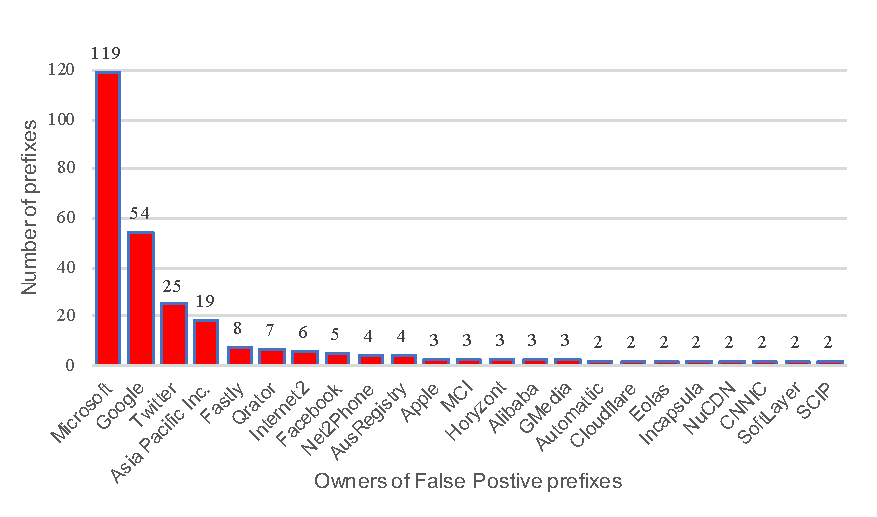
\includegraphics[scale=0.58]{fig/FP_owners.pdf}}
	\caption{Breakdown of the Owners of False Positive Prefixes}
	\label{FP_owners}
\end{figure}

%!TEX root = main_acm.tex

\section{Remote Peering in Anycast Routing}
\label{sec:rp}
The inspection of false positives suggests that remote peering might introduce unintended impact on path selection due to its invisibility at layer-3, where the direct (remote) peering at IXPs leads the local traffic to a distant location. Such a case is especially a disservice to anycast when some clients are directed to a sub-optimal replica. In this section, we attempt to identify the anycast prefixes that could be impacted by remote peering. We retrieve paths (i) towards anycast prefixes and (ii) potentially containing remote peering instances, and we validate those paths through RIPE Atlas measurements. We then perform latency measurements and present specific case studies to illustrate the practical impact of remote peering on anycast routing.

\subsection{Identifying Remote Peering in Anycast}
\label{sub:idRP}
We leverage the remote peering data from a publicly available dataset, the Remote IXP Peering Observatory \cite{RPJedi}, in which remote peering instances have been identified in 26 large IXPs worldwide.
To identify BGP paths potentially involving remote peering, first we construct
AS pairs that are connected through remote peering. We do so by pairing ASNs 
that according to \cite{RPJedi} are connected through remote peering
at an IXP ($AS_{rp}$), with the member ASNs ($AS_{mem}$)
obtained from the same IXP's website: $RP$-$AS$ $\to$ ($AS_{rp}$, $AS_{mem}$). 
We then search for such pairs in all AS paths towards anycast prefixes.\footnote{Here we use the near-ground-truth dataset (which is more conservative in labeling prefixes as anycast).} If there is any such pair appearing in the AS path of an anycast prefix, we label this prefix as potentially affected by remote peering. 

The datasets and results are shown in Table~\ref{tab_remote_data}. In all large IXPs of Europe (AMS-IX, CATNIX, DEC-IX Frankfurt, FranceIX and LINX), remote peering has the potential to affect more than 10\% of anycast prefixes. In total, there are 19.2\% (751/3,907) of anycast prefixes potentially impacted by remote peering.

\subsection{Path Collection}
To collect more information on anycast paths potentially affected by remote peering and further understand its practical impact, we conduct active measurements using the RIPE Atlas platform~\cite{RIPE_Atlas}. We select RIPE Atlas probes from the ASes that (i) host a BGP monitor and (ii) observe anycast routing paths, and perform traceroutes from the probes to the first address of anycast prefixes that are potentially affected by remote peering (\S\ref{sub:idRP}).
On average, we use 10.3 probes to traceroute a prefix. We parse the traceroute results to map each IP address to its ASN in order to obtain AS paths. Next, we look for remote peering AS pairs in these AS paths. If found, we collect and label them as paths towards prefixes potentially affected by remote peering. 

Table \ref{tab_remote_data} lists details for ASes and anycast prefixes involved
in remote peering at each IXP for which we have remote peering
data~\cite{RPJedi}. In total, we collect 1,013 AS pairs that are involved in
remote peering from 26 IXPs. We find that 751 anycast prefixes (19.2\% of total
anycast prefixes) are reached through BGP paths that include an RP-AS pair, and
we successfully traceroute 688 of them.  Since two ASes labeled as a RP-AS pair
could also peer locally at other IXPs, we then use the
traIXroute~\cite{traixroute, traixroute:pam} open-source tool to identify the
IXP crossings in the traceroutes towards these 688 prefixes, looking for IXPs
where the remote peering actually occurs. This way, we are able to confirm that
293 of these anycast prefixes are actually affected by remote peering, since
both the RP-AS pairs and the corresponding IXPs are detected in traceroutes.

We are not able to draw conclusions for the remaining 458 prefixes (out of 751), because
(1) some destination IP addresses are not reachable, (2) some intermediate IP addresses have no matching ASNs, and  (3) traIXroute~\cite{traixroute} does not include data from all IXPs where the remote peering instances have been detected. Even though these limitations lower the validation rates, we still find a significant portion of anycast prefixes that are reached through paths involving remote peering, which provides a lower bound for this phenomenon.

\begin{table}[t]
\caption{Datasets of Remote Peering. {\normalfont ({\sf \#RP}: the number of ASes involving remote peering collected from \cite{RPJedi}; {\sf \#mem-AS}: the number of IXP member ASes;  {\sf \#RP-AS}: the number of remote peering AS pairs collected from BGP information;  {\sf \#RP-Any}: the number of anycast prefixes with remote peering AS pairs (RP-AS); {\sf \%RP-Any}: percentage of anycast prefixes with RP-AS in total anycast prefixes; {\sf \#m-pfx}: the number of anycast prefixes that include RP-AS pairs in BGP paths and that can be reached by traceroute; {\sf \#v-pfx}: the number of prefixes where we validated RP-AS through traceroute.)}}
\label{tab_remote_data}
\renewcommand{\arraystretch}{1.1}
\begin{center}
\footnotesize
\begin{threeparttable}
\begin{tabular}{| p{1.2cm} p{0.6cm} p{0.6cm} p{0.7cm} | p{0.6cm} p{0.6cm} | p{0.6cm} p{0.6cm} |}
\hline
\multicolumn{1}{|c}{IXP} & {\Small\sf \#RP} & \tabincell{c}{\Small\sf \#mem\\[-1pt]-AS} & \tabincell{l}{\Small\sf \#RP\\[-1pt]-AS} & \tabincell{c}{\Small\sf {\bf \#}RP\\[-1pt]-Any} & \tabincell{c}{\Small\sf {\bf \%}RP\\[-1pt]-Any} & \tabincell{c}{\Small\sf \#m-\\[-1pt]pfx} & \tabincell{c}{\Small\sf \#v-\\[-1pt]pfx} \\[3pt]
\hline
AMS-IX & 355 & 821 & 758 & 608 & 15.83 & 545 & 165 \\
BIX & 9 & 65 & 1 & 1 & 0.026 & 1& 0 \\
BIX.BG  & 17 & 79 &  0 & 0 & 0 & -& -\\
CABASE{\textsuperscript{\dag}}  & 15 & 71 & 0  & 0 & 0 & -& -\\
CATNIX & 9 & 42 & 7 & 568 & 14.78 & 568 & 5 \\
DE-CIX Fr{\textsuperscript{\ddag}} & 367 & 826 & 383 & 520 & 13.53 & 520 & 182 \\
FICIX  & 4 &  34 & 3 & 35 & 0.91 & 35 & 0 \\
France-IX{\textsuperscript{$\natural$}}  & 118 & 369 & 147 & 388 & 10.10 & 326 & 71 \\
HKIX & 46 & 288 & 15 & 85 & 2.21 & 85 & 38 \\
IIX  & 92 & 222 & 0 & 0 & 0 & -& -\\
INEX  & 11 & 101 &0 & 0 & 0 &- & -\\
QLD-IX  & 4 & 81 & 2 & 31 & 0.81 &31 & 31 \\
IX Man{\textsuperscript{$\sharp$}} & 12 & 95 & 5 & 65 & 1.69 & 65 & 0 \\
LINX LON1 & 151 & 787 & 224  & 511 & 13.30 & 511 & 140 \\
LINX NoVA & 9 & 45 & 5 & 36 & 0.94 & 36 & 0 \\
LONAP & 13 & 200& 13 & 83 & 2.16 & 83 & 60\\
MIX-IT  & 49 & 241 & 26& 237 & 6.17 & 237 & 43 \\
NIX.CZ & 32 & 152 & 17 & 66 & 1.71 & 66 & 0 \\
SGIX& 8 & 96 & 0 & 0 & 0 & -& -\\
SIX.SK & 4 & 57 & 0 & 0 & 0 &-& -\\
SwissIX  & 48 & 185 & 78 & 135 & 3.51 & 147 & 91 \\
Thinx  & 29 & 183 & 2 & 9 & 0.23 & 9 & 0 \\
TPIX & 33 & 220 &0 & 0 & 0 & -& -\\
TPIX-TW & 4 & 41 & 1 & 6 & 0.16 & 6 & 0 \\ 
UA-IX  & 38 & 189 & 0 & 0 & 0 & -& -\\
VIX & 32 & 140 &  17 &  97 & 2.52 & 97 & 30\\
\hline
Total\textsuperscript{\P}  & 1,075 & 3,377 & 1,013 &  751 & 19.2 & 688 & 293 \\
\hline
\end{tabular}
\begin{tablenotes}
{\SMALL
      \item {{\textsuperscript{\dag}CABASE-BUE-IX Argentina; \ } {\textsuperscript{\ddag}DE-CIX Frankfurt; \ } {\textsuperscript{$\natural$}France-IX Paris; \ } {\textsuperscript{$\sharp$}IX Manchester}}
      \item {\textsuperscript{\P}We remove the duplicated prefixes.}}
\end{tablenotes}
%\vspace{-3pt}
\end{threeparttable}
\end{center}
\end{table}

\subsection{Impact of Remote Peering: Performance Analysis and Case Study}
Leveraging the traceroute experiments we used in \S3.2, we study the impact of remote peering by analyzing the performance and route selection in real-world case studies.

\vspace{3pt}
\textbf{Performance Analysis and Case Study.}
To quantify the performance impact of remote peering on anycast path selection, 
we measure the round-trip time (RTT) to each
anycast prefix from the same measurements collected in \S5.2. Among the
successful traceroutes, we find that 38\% (126/332) of RTTs in traceroutes
towards anycast prefixes potentially affected by remote peering are larger than
the average RTT of prefixes without remote peering.
In these 126 traceroute probes, the average RTT towards prefixes potentially affected by remote peering is 119.7 ms while the average RTT of the other prefixes is 84.7 ms. An average latency increase of 35.1 ms. 

In a concrete example, we traceroute to the IP address of the DNS D-root from a probe located in Singapore.
Ideally, we expect that our traceroute can reach the D-root instance in Singapore~\cite{RootDNS}.
However, we found that the traceroute goes to Europe via AMS-IX and through
remote peering, and reach another D-root server in Amsterdam, Netherlands, with a 158 ms RTT. Consequently, remote peering not only can affect performance, but it may also impact traffic engineering or load balancing, potentially routing traffic through to unintended locations.

%\textbf{Case Study.} We then provide concrete cases from the path collection experiments to illustrate practical impact. For example, we found that for a traceroute-targeted IP address \texttt{\small 103.245.222.1} (i.e., the first address of the anycast prefix \texttt{\small 103.245.222.0/24}),
%located in @@@@IS IT UNICAST INSTEAD??@@@@ Frankfurt, Germany, the traceroute from one of our probes in Eastern US (Ashburn, VA) first went to San Jose, CA in Western US, then traveled to Hong Kong, and finally arrived in Frankfurt, Germany. This happened because a remote peering AS pair at DECIX, AS3491 and AS2914, produced a short AS path but it routed traffic through geographically distant locations, while actually shorter routes (but appearing as longer AS paths) were announced. Note that this case is similar to the impact of remote peering on unicast.

%Consequently, we can see that remote peering can affect the route selection and performance as well as traffic engineering and load balancing, potentially routing traffic through to unintended locations. 

\vspace{3pt}
\textbf{DNS Root Sever Anycast Data}. 
We conduct an extensive study using a dataset of traceroutes towards anycast addresses provided by University of Maryland (UMD)~\cite{UMD_anycast}, which includes  traceroute data from selected probes to C-, D- and K-DNS root server sites. By searching for IPs/ASes involving remote peering in  paths towards such anycast addresses, we identify remote peering in D and K root server traces. Specifically, we find remote peering instances located in AMS-IX and DECIX from D-root experiments, and SIX.SK, FranceIX Paris, AMS-IX and Linx from K-root experiments.
These results are consistent with our previous results in \S5.2. 

Also in the UMD dataset, we find specific cases where remote peering affects
anycast routing by taking traffic on geographically-long routes. For example, we
observed that traceroutes from probes in Eastern Russia were routed to
Netherlands and Germany, respectively, through routes with remote peering, while
there are root DNS server instances in Hong Kong and Tokyo. These cases confirm
the observations from Li et al. in~\cite{li2018internet}, in which the same
dataset has been used to study the inefficiency of anycast path selection, and
explain the reason why some users cannot reach the optimal DNS root sites
(although the work from Li et al. does not mention remote peering among potential causes).


%!TEX root = main_acm.tex

\section{Related Work}
\label{sec:rel}
Anycast deployment and performance have been characterized and evaluated by different active probing methods. Madory \emph{et al.}~\cite{madory2013anycasters} use geolocation of transit IP and geo-inconsistency to detect anycast prefixes. Cicalese \emph{et al.} ~\cite{cicalese2015characterizing, cicalese2015fistful, cicalese2018longitudinal} propose a method for enumeration and geolocation of anycast instances based on latency measurements. Vries \emph{et al.}~\cite{deVries:2017} propose a method that maps anycast catchments via active probes to provide better coverage. 

\textbf{Anycast-based Internet Services}.
Fan \emph{et al.} ~\cite{fan2013} combine the CHAOS queries with traceroutes and use new IN records to support open recursive DNS servers as vantage points to detect and study anycast-based DNS infrastructures.
Calder \emph{et al.} ~\cite{Calder:2015} study the performance of an anycast CDN and find that some clients are directed to a sub-optimal front-end.
Moura \emph{et al.} ~\cite{moura2016anycast} study the Nov. 2015 event of Root DNS attacked by DDoS from the anycast's perspective. 
Giordano \emph{et al.}~\cite{giordano2016first} perform a passive characterization study on anycast traffic in CDNs and present temporal properties, service diversity, and deployments of anycast traffic.

Schmidt \emph{et al.} ~\cite{de2017anycast} investigate the relationship between IP anycast and latency from four Root DNS nameservers. Their key results show that geographic location and connectivity have a stronger impact on latency than the number of sites. 
Li \emph{et al.}~\cite{li2018internet} perform a study on anycast's route selection and performance using D-root Server traces, and they validate that equal-length AS paths are the main reason for anycast latency inflation.
Wei \emph{et al.}~\cite{wei2018does} study the service (in)stability of anycast services. They confirm that a small number of users are affected by the instability of anycast, potentially caused by the load balancers on the path.

\textbf{Remote Peering}.
Castro \emph{et al.}~\cite{castro2014remote} present a systematic study of remote peering at IXPs using ping-based methods. They discuss the impact of remote peering on Internet reliability, security, and economies.
Nomikos \emph{et al.}~\cite{Nomikos18} perform a comprehensive measurement study
of remote peering, and they achieve very high accuracy and coverage levels by
combining RTT measurements with other domain-specific information like facility
locations, IXP port capacity, and private connectivity. They study the features
and trends of remote peering, showing that remote peering may route traffic to
more distant destinations. Their work does not focus on anycast prefixes though.


%!TEX root = main_acm.tex

\section{Conclusion}
\label{sec:con}

We presented a passive method to study IP anycast by utilizing BGP data.  We
proposed a set of BGP-related features (thus not based on active measurements)
to classify anycast and unicast prefixes. Extracting data from RouteViews and
RIPE RIS, we evaluated the effectiveness of our proposed approach against a
near-ground-truth dataset based on active-probing
measurements~\cite{cicalese2015characterizing}. The evaluation results show that
our approach achieves high classification accuracy---about 90\% for anycast and
99\% for unicast---and is also able to detect anycast prefixes incorrectly
labeled as unicast in the near-ground-truth dataset. 

In addition, while delving into the causes of inaccuracy, we found indication
that remote peering might have an unintended impact on anycast routing. We
investigated this phenomenon by combining regular traceroutes, measurements
executed with the traIXroute~\cite{traixroute, traixroute:pam} open-source tool,
BGP data from RouteViews and RIPE RIS, and data from the Remote IXP Peering
Observatory \cite{RPJedi}.  Our study showed that remote peering has the
potential to affect 19.2\% of the anycast prefixes and we confirmed via
traceroute measurements that around 40\% of such prefixes were indeed impacted
by remote peering.  We also revealed that remote peering could increase
transmission latency by routing traffic to distant suboptimal anycast sites.



\begin{acks}
We would like to thank our Editor, Olivier Bonaventure, as well as Ignacio Castro and the anonymous reviewers for their insightful comments. We would also like to thank Vasileios Giotsas and Dave Levin for sharing their datasets. This work was supported by National Science Foundation grants CNS-1618117, CNS-1705024, and DGE-1821744.
This material is also based on research sponsored by Air Force Research Laboratory under agreement number FA8750-18-2-0049. The U.S. Government is authorized to reproduce and distribute reprints for Governmental purposes notwithstanding any copyright notation thereon. The views and conclusions contained herein are those of the authors and should not be interpreted as necessarily representing the official policies or endorsements, either expressed or implied, of Air Force Research Laboratory or the U.S. Government.
\end{acks}

\bibliographystyle{ACM-Reference-Format}
%\bibliographystyle{abbrv}
\bibliography{bibliography}

\end{document}

